\documentclass{beamer}

\usepackage{beamerthemesplit}
\usepackage{graphicx}
\usepackage{subfigure}
\usepackage{amsmath,amssymb}
\usepackage{multimedia}
\usepackage{times}

\usepackage[latin1]{inputenc}
\usepackage[T1]{fontenc}
\usepackage{listings}
\usepackage{courier}
\usepackage{color}
\usepackage{rotating}

\newcommand{\re}{\text{Re}}
\newcommand{\im}{\text{Im}}
\newcommand{\de}{\mbox{d}}
\newcommand{\eref}[1]{(\ref{#1})}
\newcommand{\ii}{\text{i}}
\newcommand{\ee}{\text{e}}
\newcommand{\mathbi}[1]{\textbf{\em #1}}
\newcommand{\rem}[1]{}

% \newcommand{\heading}[1]{\centerline{\Large #1} \vspace{0.5em}}
\newcommand{\heading}[1]{\frametitle{#1}}

\newcommand{\odeint}[0]{odeint}
\newcommand{\thrust}[0]{Thrust}
\newcommand{\vexcl}[0]{VexCL}
\newcommand{\boostcompute}[0]{Boost.Compute}
\newcommand{\viennacl}[0]{ViennaCL}
\newcommand{\cmtl}[0]{Cuda-MTL4}



% Layout specification

% \usetheme{AnnArbor}
% \usetheme{Antibes}
% \usetheme{Bergen}
% \usetheme{Berkeley}
% \usetheme{Berlin}
% \usetheme{Boadilla}
% \usetheme{boxes}
% \usetheme{CambridgeUS}
% \usetheme{Copenhagen}
% \usetheme{Darmstadt}
% \usetheme{default}
% \usetheme{Dresden}
% \usetheme{Frankfurt}
% \usetheme{Goettingen}
% \usetheme{Hannover}
% \usetheme{Ilmenau}
% \usetheme{JuanLesPins}
% \usetheme{Luebeck}
% \usetheme{Madrid}
% \usetheme{Malmoe}
% \usetheme{Marburg}
% \usetheme{Montpellier}
% \usetheme{PaloAlto}
% \usetheme{Pittsburgh}
% \usetheme{Rochester}
% \usetheme{Singapore}
% \usetheme{Szeged}
\usetheme{Warsaw}

% \usecolortheme{albatross}
% \usecolortheme{beaver}
% \usecolortheme{beetle}
% \usecolortheme{crane}
% \usecolortheme{default}
% \usecolortheme{dolphin}
% \usecolortheme{dove}
% \usecolortheme{fly}
% \usecolortheme{lily}
% \usecolortheme{orchid}
% \usecolortheme{rose}
% \usecolortheme{seagull}
% \usecolortheme{seahorse}
% \usecolortheme{sidebartab}
% \usecolortheme{structure}
% \usecolortheme{whale}
% \usecolortheme{wolverine}

% \usefonttheme{default}
% \usefonttheme{professionalfonts}
% \usefonttheme{serif}
% \usefonttheme{structurebold}
% \usefonttheme{structureitalicserif}
% \usefonttheme{structuresmallcapsserif}

% \useinnertheme{circles}
% \useinnertheme{default}
% \useinnertheme{inmargin}
% \useinnertheme{rectangles}
% \useinnertheme{rounded}

% \useoutertheme{default}
% \useoutertheme{infolines}
% \useoutertheme{miniframes}
% \useoutertheme{shadow}
% \useoutertheme{sidebar}
% \useoutertheme{smoothbars}
% \useoutertheme{smoothtree}
% \useoutertheme{split}
% \useoutertheme{tree}






% Meta

\title[Iteratorst]{Iterators and Ranges for numerical problems}
% \subtitle[Iterators]{Solving ordinary differential equations in C++}
\author[Karsten Ahnert]{Karsten Ahnert}
\institute[Ambrosys]{Ambrosys GmbH, Potsdam}
\date{\today}
%\logo{\pgfimage[width=2cm,height=2cm]{logo}}
\titlegraphic{\includegraphics[width=4cm]{ambrosys}}
\subject{Subject}
\keywords{Keyword1,Keyword2}

\newcommand{\sectionslide}[1]{\frame{\begin{centerline}{\LARGE #1}\end{centerline}}}




\definecolor{dark-gray}{gray}{0.15}
\definecolor{light-gray}{gray}{0.8}
\definecolor{lighter-gray}{gray}{0.9}

\definecolor{dark-green}{rgb}{0,0.4,0}
\definecolor{dark-red}{rgb}{0.2,0,0}

\newcommand{\highlight}[1]{\bf #1}

\lstset{
         basicstyle=\small\ttfamily, % Standardschrift
         %numbers=left,               % Ort der Zeilennummern
         numberstyle=\tiny,          % Stil der Zeilennummern
         %stepnumber=2,               % Abstand zwischen den Zeilennummern
         numbersep=0pt,              % Abstand der Nummern zum Text
         tabsize=2,                  % Groesse von Tabs
         extendedchars=true,         %
         breaklines=true,            % Zeilen werden Umgebrochen
         frame=single,         
         backgroundcolor=\color{lighter-gray},
         tabsize=2,
         keywordstyle=\color{dark-green},
         identifierstyle=,
         commentstyle=\color{dark-gray}\normalfont\rmfamily\itshape,
         stringstyle=\color{dark-red},
         showspaces=false,           % Leerzeichen anzeigen ?
         showtabs=false,             % Tabs anzeigen ?
         xleftmargin=10pt,
         xrightmargin=10pt,
         framexleftmargin=5pt,
         framexrightmargin=5pt,
         framexbottommargin=4pt,
         language=c++,
         showstringspaces=false      % Leerzeichen in Strings anzeigen ?        
 }
\lstloadlanguages{C++}


% What is shown

\beamertemplatenavigationsymbolsempty
\setbeamertemplate{footline}{}
%\setbeamertemplate{footline}{\insertframenumber}
\setbeamertemplate{headline}{}

\setbeamercolor{palette quaternary}{fg=black,bg=white}
\setbeamerfont{frametitle}{size=\Large}
\setbeamercolor{frametitle}{parent=palette quaternary}
\setbeamertemplate{frametitle}
{
  \vspace{1ex}
  \begin{beamercolorbox}[ht=2ex,wd=\paperwidth]{frametitle}
    \centerline{\insertframetitle}
  \end{beamercolorbox}
}

\parindent0pt


\begin{document}



\frame{
  \titlepage


}

\begin{frame}
  \heading{Outline}

  \tableofcontents
\end{frame}

\section{Introduction}

\sectionslide{Introduction}

\frame{
  \heading{Iterators}
  
  Unique way to traverse containers
  
  Unique way to apply iterative IO
  
  Unique way of expressing algorithms
}

\begin{frame}[fragile]{Example}
 \heading{Example -- basic use}
 \begin{lstlisting}[basicstyle=\scriptsize\ttfamily]
 for( auto iter = values.begin() ;
      iter != values.end() ;
      ++iter )
 {
     cout << *iter << endl;
 }
 \end{lstlisting}
 \pause

 \vspace{2ex}
 C++11 - use range based for
 \begin{lstlisting}[basicstyle=\scriptsize\ttfamily]
  for( auto v : values )
  {
      cout << v << endl;
  }
 \end{lstlisting}

\end{frame}



\begin{frame}[fragile]
 \heading{Example -- Container traversal}
 \begin{onlyenv}<1>
 \begin{lstlisting}
  list< double > values;
  list< double > values2( values.size() );
 \end{lstlisting}
 \end{onlyenv}
 \begin{onlyenv}<2>
 \begin{lstlisting}
  vector< double > values;
  vector< double > values2( values.size() );
 \end{lstlisting}
 \end{onlyenv} 
 \vspace{2ex}
 Can be used in
 \begin{lstlisting}
  transform( values.begin() , values.end() ,
             values2.begin() ,
             []( double x ) {
                 return x * 2.0; } );
 \end{lstlisting}
\end{frame}




\begin{frame}[fragile]
  \heading{Examples -- IO}

Input
\begin{lstlisting}[basicstyle=\scriptsize\ttfamily]
vector< double > values;  
copy_if( istream_iterator< double >( cout ) ,
         istream_iterator< double >() ,
         back_inserter( values ) ,
         []( double x ) { return x > 0.0; } );
\end{lstlisting}
\vspace{2ex}
Output
\begin{lstlisting}[basicstyle=\scriptsize\ttfamily]
vector< double > values;  
// fill values
copy_if( values.begin() , values.end() ,
         ostream_iterator< double >( std::cout , "\n" ) ,
         []( double x ) { return x > 0.0; } );
\end{lstlisting}

\end{frame}


\begin{frame}[fragile]
 \heading{Examples -- Combine algorithms}
 
 Find a nice real life example.
\end{frame}



\frame{
  \heading{Iterator types -- Concepts}
  
  \centerline{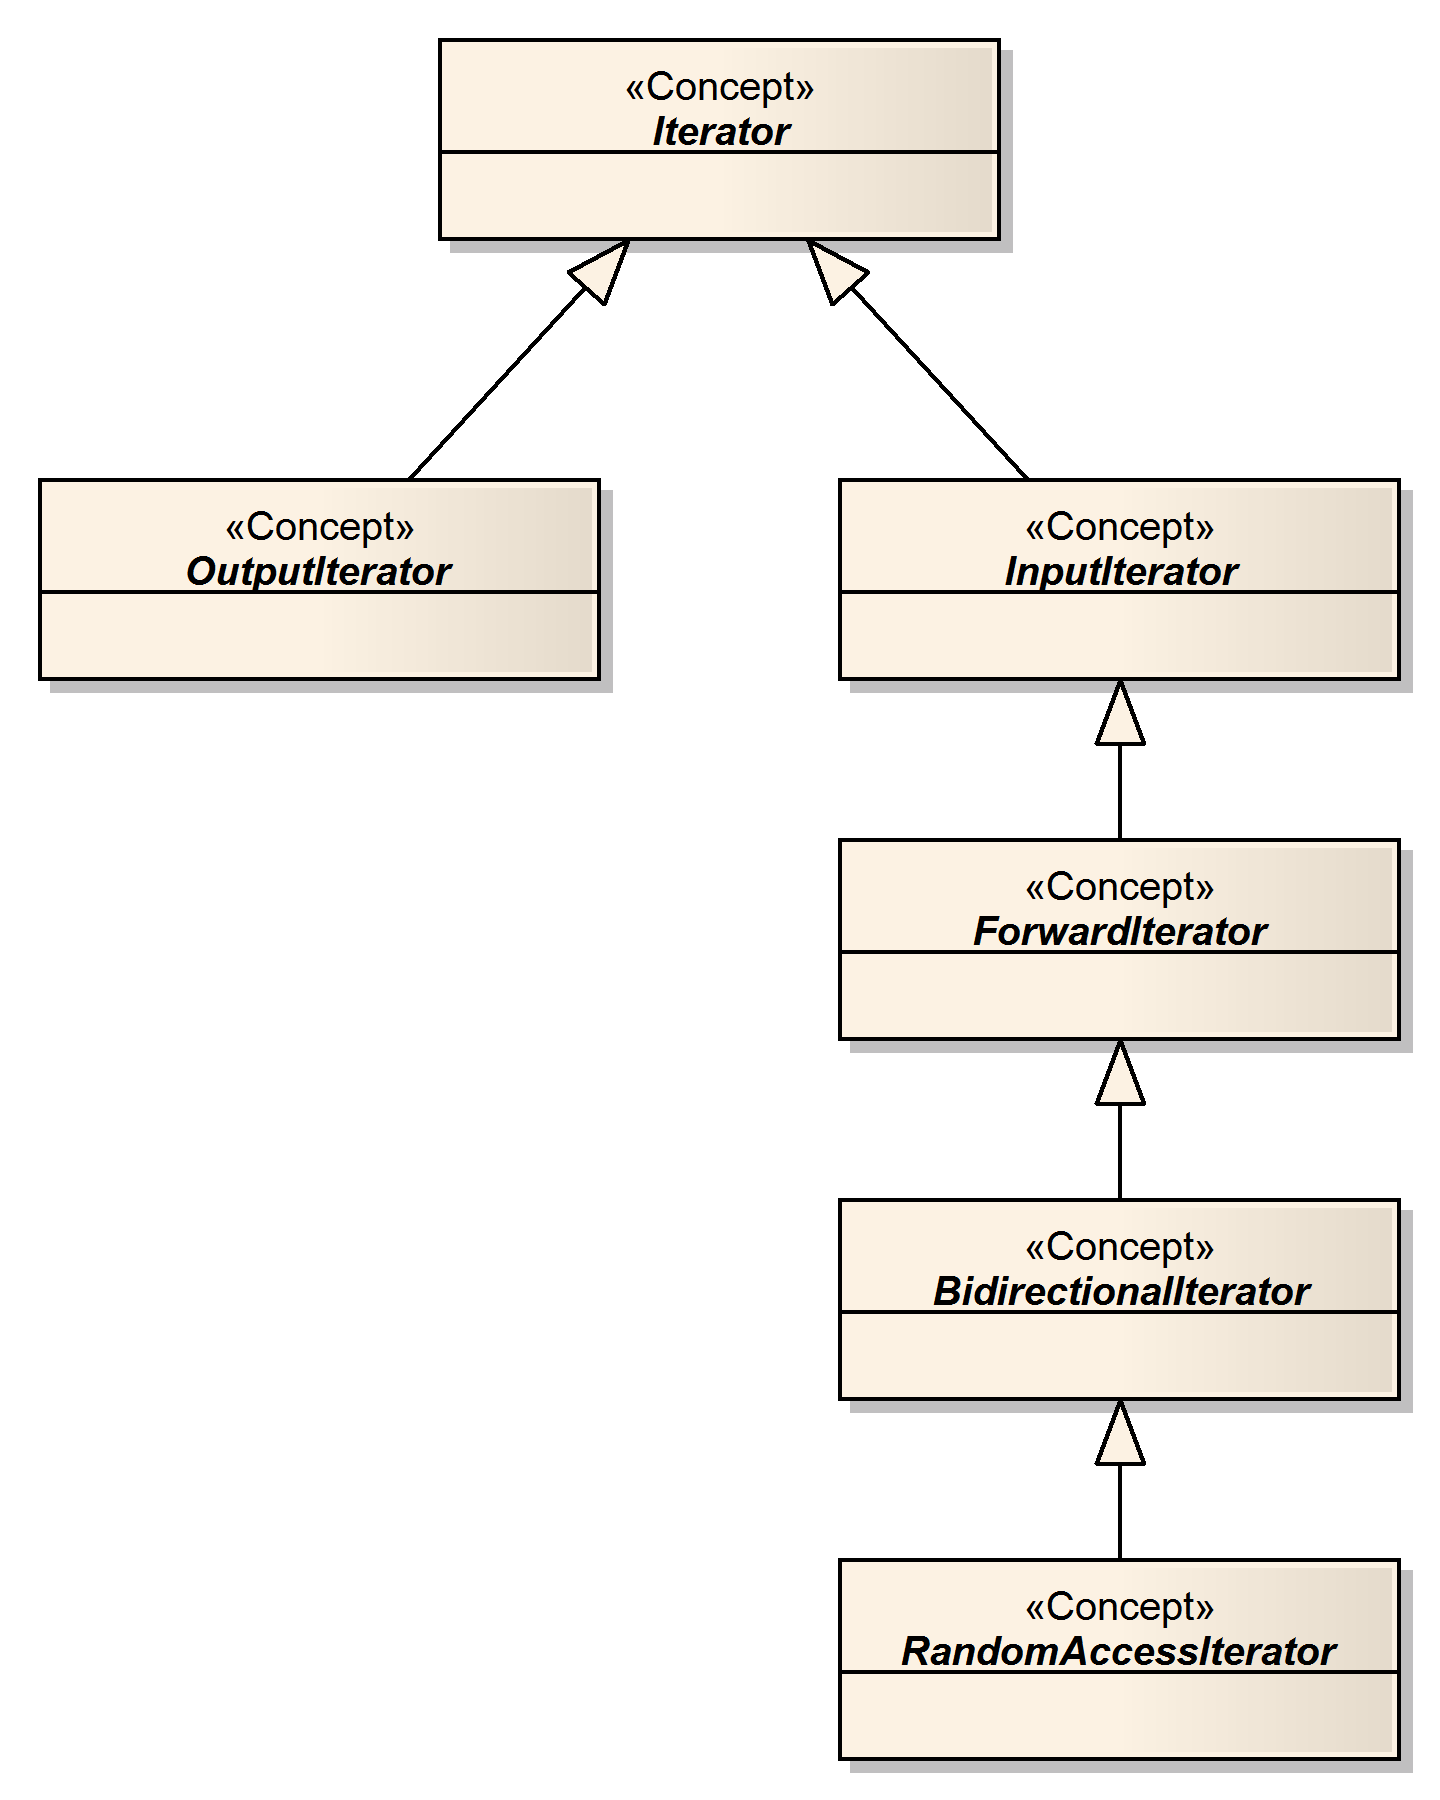
\includegraphics[width=0.5\textwidth]{IteratorsOverview}}
}

\begin{frame}[fragile]
  \heading{Iterator types -- Concepts}
  
  \vspace{2ex}
  
  \begin{columns}[T]
    \begin{column}{0.45\textwidth}
      \centerline{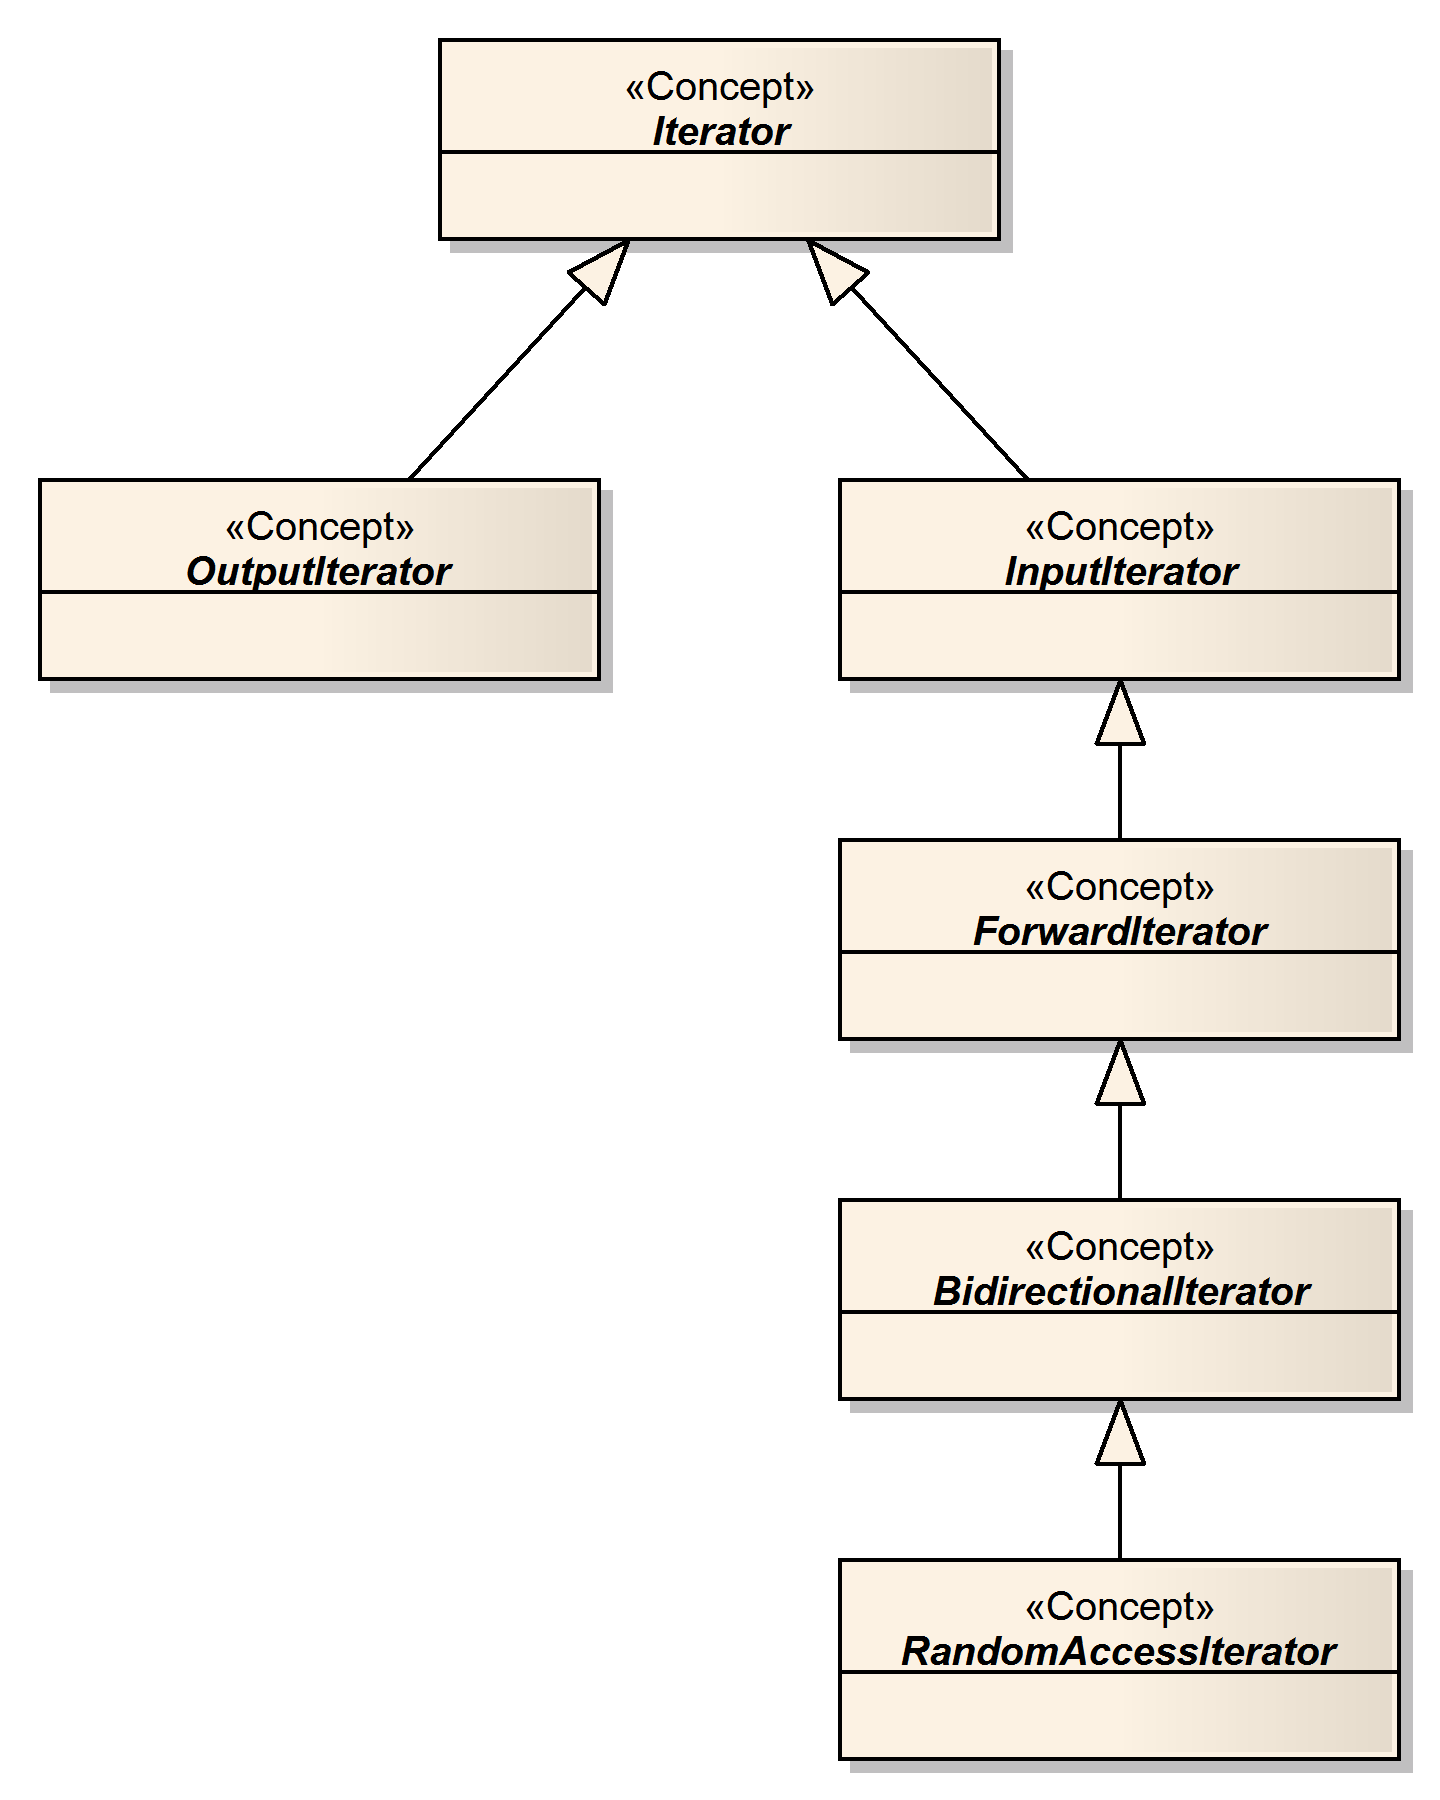
\includegraphics[width=1.0\textwidth]{IteratorsOverview}}
    \end{column}
    \begin{column}{0.55\textwidth}
      \begin{onlyenv}<1>
         OutputIterator
         
         \begin{lstlisting}
*i = o;
*i++ = o;
i++;
++i;
         \end{lstlisting}

         Are special, {\tt back\_inserter}, {\tt ostream\_iterator}, ...
      \end{onlyenv}
      \begin{onlyenv}<2>
         InputIterator a.k.a. Single-Pass Iterator
         
         \begin{lstlisting}
bool r = i != j;
val x = *i;
iterator j = ++i;
i++;
val x = *i++;
         \end{lstlisting}
{\tt istream\_iterator}, {\tt istreambuf\_iterator}

          \vspace{2ex}
          But, if {\tt i == j} then {\tt ++i != ++j}
      \end{onlyenv}
      \begin{onlyenv}<3>
         ForwardIterator
         \begin{lstlisting}
iterator j = i++;
         \end{lstlisting}

          \vspace{2ex}
          But, if {\tt i == j} then {\tt ++i == ++j}
      \end{onlyenv}
      \begin{onlyenv}<4>
         BidirectionalIterator
         \begin{lstlisting}
iterator j = --i;
iterator j = i--;
val x = *i--;
         \end{lstlisting}
         {\tt map< K , V >::iterator, list< T >::iterator}
      \end{onlyenv}
      \begin{onlyenv}<5>
         RandomAccessIterator
         \begin{lstlisting}
i += n;
i -= n;
val x = i[n];
long dist = i - j;
bool b = i < j;
         \end{lstlisting}
         {\tt vector< T >::iterator}
      \end{onlyenv}
    \end{column}
  \end{columns}
\end{frame}




\frame{
  \heading{Algorithms}
  \tiny \tt
  \begin{columns}[T]
   \begin{column}{0.2\textwidth}
      \hrule
      I all\_of \\
      I any\_of \\
      I none\_of \\
      I for\_each \\
      I count \\
      I count\_if \\
      I mismatch \\
      I equal \\
      I find \\
      I find\_if \\
      I find\_if\_not \\
      F find\_end \\
      I,F find\_first\_if \\
      F adjacent\_find \\
      F search \\
      F search\_n \\
      \hrule
      I,O copy \\
      I,O copy\_if \\
      I,O copy\_n \\
      B,O copy\_backward \\
      I,O move \\
      B,O move\_backward \\
      F fill \\
      F fill\_n \\
      I,O transform \\
      F generate \\
      I generate\_n \\
   \end{column}
   \begin{column}{0.2\textwidth}
      F remove \\
      F remove\_if \\
      I,O remove\_copy \\
      I,O remove\_copy\_if \\
      F replace \\
      F replace\_if \\
      I,O replace\_copy \\
      I,O replace\_copy\_if \\
      F swap\_ranges \\
      F iter\_swap \\
      B reverse \\
      B,O reverse\_copy \\
      F rotate \\
      F,O rotate\_copy \\
      R random\_shuffle \\
      R shuffle \\
      F unique \\
      I,O unique\_copy
   \end{column}
   \begin{column}{0.3\textwidth}
     \hrule
     I is\_partitioned \\
     F,B partition \\
     I,O partition\_copy \\
     B stable\_partition \\
     F partition\_point \\
     F is\_sorted \\
     F is\_sorted\_until \\
     R sort \\
     R partial\_sort \\
     I,R partial\_sort\_copy \\
     R stable\_sort \\
     R nth\_element \\
     \hrule
     F lower\_bound \\
     F upper\_bound \\
     F binary\_search \\
     F equal\_range \\
     I,O merge \\
     B inplace\_merge \\
     I includes \\
     I,O set\_difference \\
     I,O set\_intersection \\
     I,O set\_symmetric\_difference \\
     I,O set\_unition 
   \end{column}
   \begin{column}{0.3\textwidth}
     \hrule
     R is\_heap \\
     R is\_heap\_until \\
     R make\_heap \\
     R push\_heap \\
     R pop\_heap \\
     R sort\_heap \\
     \hrule
     F max\_element \\
     F min\_element \\
     F minmax\_element \\
     I lexicographical\_compare \\
     F is\_permutation \\
     B next\_permutation \\
     B prev\_permutation \\
     \hrule
     F iota \\
     I accumulate \\
     I inner\_product \\
     I,O adjacent\_difference \\
     I,O partial\_sum
   \end{column}
  \end{columns}


}


\begin{frame}[fragile]
  \heading{Ranges}
  
  Simplifying iterators
  
  Generalization of iterators
  
  First defined in Boost
  
  Soon in the standard library?

  \begin{lstlisting}
vector< double > values;
boost::for_each( values , []( double x ) { cout << x << endl; } );
  \end{lstlisting}


\end{frame}


\frame{
 \heading{Ranges -- more examples from boost}
 
 Filters
 
 complicated algorithms
}



\frame{
  \heading{Ranges in Boost}
  
  Ranges are pairs of iterators.
  
  Memory overhead
  
  Filters grow exponential in size
}

\frame{
  \heading{Ranges for the native C++}
  
  The range is the main abstraction not the iterator
  
  It holds all informations
  
  Concepts, asymmetric algorithms, sentinels have their own type.
}



\section{Iterators and ranges for dynamical systems}

\sectionslide{Iterators and ranges for dynamical systems}

\begin{frame}[fragile]
  \heading{Dynamical systems -- Maps}
  
  \begin{displaymath}
   x_{n+1} = f( x_n )
  \end{displaymath}
  
  \begin{onlyenv}<1>
  picture of logistic map
  \end{onlyenv}
  \begin{onlyenv}<2>
     Iota:
     
     \begin{lstlisting}
std::iota( first , last , 1 );
     \end{lstlisting}
     
     $$x_{n+1} = x_n + 1 \quad\quad ( 1 , 2 , 3 , 4 , \dots )$$
     
     Generalized iota:
     
     $$x_{n+1} = x_n + 2 \quad \quad ( 1 , 3 , 5 , 7 , \dots )$$
     
     $$x_{n+1} = 2 x_n \quad \quad ( 1 , 2 , 4 , 8 , \dots )$$
     
     $$x_{n+1} = x_n^2 \quad \quad ( 1 , 1 , 1 , 1 , \dots )$$
  \end{onlyenv}
\end{frame}

\frame{
  \heading{Dynamical systems -- ODEs}
  
  \begin{displaymath}
   \frac{\de x}{\de t} = f( x , t )
  \end{displaymath}
  
  picture of lorenz system?
}

\frame{
  \heading{Numerical integration}

  Lagrange integration
}


\frame{
  \heading{Map iterator}
  
  Abstraction for $x_{n+1} = f(x_n)$
  
  Problems:
  
  \begin{enumerate}
   \item $x$ could be intrinsic state of the iterator, or the iterator iterates $x$.
   \item Stop criterium, which is the end iterator
  \end{enumerate}
}

\frame{
  \heading{Map iterator}
  
  Implementation
  
  two flavours, with count, with predicate
  
  Naive implementation
}


\frame{
  \heading{Map iterator - applications}
  
  Generalized iota
  
  Functional random number generators
  
  
}

\frame{
  \heading{Map iterator - pros and cons}
  
  Pro:
  \begin{itemize}
   \item Generalization of dynamical systems
  \end{itemize}

  Contra:
  \begin{itemize}
   \item end iterators needs to be unnecessary complex
  \end{itemize}
}



\frame{
  \heading{Map range}
  
  Better implementation
}

\frame{
  \heading{Map iterators and ranges for the new standard}
  
  Sentinels
}

\section{Iterators for GPUs}

\sectionslide{Iterators for GPUs algorithms}

\frame{
  \heading{High-level libraries for GPUs}
  
  \begin{enumerate}
    \item Thrust
    \item VexCL
    \item Boost.Compute
    \item ViennaCL
    \item Cuda-MTL
  \end{enumerate}
}

\frame{
  \heading{Thrust}
  
  STL-like library for Cuda
  
  Design is based on iterators
}

\frame{
  \heading{Iterators in Thrust}
  
  {\tt device\_vector::iterator}
  
  {\tt host\_vector::iterator}
  
  special iterators
  
  Algorithms
}

\frame{
  \heading{Implementation details of Thrust iterators}

}

\frame{
  \heading{Special iterators for Thrust}
  
  zip iterator
  
  transform iterator
  
}

\frame{
  \heading{Special problems - and solutions}

  Norm
}

\frame{
  \heading{Special problems - and solutions}
  
  Bucket sort
}


\frame{
  \heading{Solving an ensemble of low-dimensional ODEs}
  
  Lorenz example and ODEs
}

\section{Conclusion}

\frame{
  \heading{Conclusion}
  
  
}

\frame{
  \heading{Outlook}
}


\frame{
  \heading{References}
}


\end{document}
